\hypertarget{v6.1-ux72ecux7acbux786eux8ba4ux590dux73b0ux4e0e-frozen-test}{%
\section{V6.1 独立确认、复现与 frozen test}\label{v6.1-ux72ecux7acbux786eux8ba4ux590dux73b0ux4e0e-frozen-test}}

\hypertarget{ux72ecux7acb-300-episode-paired-confirmation}{%
\subsection{独立 300-episode paired confirmation}\label{ux72ecux7acb-300-episode-paired-confirmation}}

confirmation 使用 seeds \texttt{7,000,000–7,000,299} 的 300 个全新 episode。E0、E2 和 Oracle 使用完全相同的 episode IDs 与 initial seeds；逐 episode outcome 被保存，因此 E2--E0 可以计算 paired wins/losses/ties、bootstrap confidence interval 和 exact McNemar 检验。

\begin{longtable}[]{@{}
  >{\raggedright\arraybackslash}p{(\columnwidth - 8\tabcolsep) * \real{0.1579}}
  >{\raggedleft\arraybackslash}p{(\columnwidth - 8\tabcolsep) * \real{0.2105}}
  >{\raggedleft\arraybackslash}p{(\columnwidth - 8\tabcolsep) * \real{0.2105}}
  >{\raggedleft\arraybackslash}p{(\columnwidth - 8\tabcolsep) * \real{0.2105}}
  >{\raggedleft\arraybackslash}p{(\columnwidth - 8\tabcolsep) * \real{0.2105}}@{}}
\toprule\noalign{}
\begin{minipage}[b]{\linewidth}\raggedright
Policy
\end{minipage} & \begin{minipage}[b]{\linewidth}\raggedleft
Benchmark
\end{minipage} & \begin{minipage}[b]{\linewidth}\raggedleft
Strict
\end{minipage} & \begin{minipage}[b]{\linewidth}\raggedleft
Exit/Entry
\end{minipage} & \begin{minipage}[b]{\linewidth}\raggedleft
20-step hold
\end{minipage} \\
\midrule\noalign{}
\endhead
\bottomrule\noalign{}
\endlastfoot
E0 & 157/300（52.3\%） & 81/300（27.0\%） & 93/157（59.2\%） & 118/300（39.3\%） \\
E2 & 205/300（68.3\%） & 111/300（37.0\%） & 120/205（58.5\%） & 170/300（56.7\%） \\
Oracle & 194/300（64.7\%） & 109/300（36.3\%） & 99/194（51.0\%） & 169/300（56.3\%） \\
\end{longtable}

E2 相对 E0 的 Benchmark 提升 16 percentage points：66 个 episode 仅 E2 成功，18 个仅 E0 成功，216 个同结果；paired 95\% bootstrap CI 为 \texttt{{[}+10.33,+21.67{]}pp}，exact McNemar \texttt{p=1.33×10\^{}-7}。Strict 提升 10pp：60 wins、30 losses、210 ties，paired CI \texttt{{[}+4,+16{]}pp}，\texttt{p=0.00206}。因此可以明确写出：\textbf{固定 E2 在独立 300-episode paired simulation confirmation 上显著提高 Benchmark 与 Strict。}

E2 在该 bank 上名义高于 Oracle 3.7pp Benchmark、0.7pp Strict，但这不是``视觉策略普遍超过 Oracle''的证据。Oracle 在旧 100-episode开发 bank 为 75\% / 42\%，在新 bank 为 64.7\% / 36.3\%，显示有限样本和初始状态组合会改变名义排序。E2 的状态误差也可能偶然形成对某些 root 有利的 controller bias。严谨说法是：E2 在这一个独立 bank 上达到接近 Oracle 的闭环水平，同时显著优于同初始状态的 E0。

Exit/Entry 从 E0 的 59.2\% 到 E2 的 58.5\%，没有明显恶化；但 E2 entry 数从 157 增至 205，条件分母不同，不能把 0.7pp 的下降当作直接 hold 因果证据。更强的证据是 20-step hold 从 118/300 增至 170/300，以及下一节在相同 first-entry root 上的固定入口比较。

\hypertarget{fixed-entry-hold}{%
\subsection{Fixed-entry hold}\label{fixed-entry-hold}}

固定入口实验从 200 个共同的 E0 first-entry roots 恢复 E0、E2 和 Oracle，避免不同策略 entry 数量带来的分母混淆：

\begin{longtable}[]{@{}lrr@{}}
\toprule\noalign{}
Policy & 20-step survival & 50-step survival \\
\midrule\noalign{}
\endhead
\bottomrule\noalign{}
\endlastfoot
E0 & 123/200（61.5\%） & 100/200（50.0\%） \\
E2 & 123/200（61.5\%） & 94/200（47.0\%） \\
Oracle & 129/200（64.5\%） & 106/200（53.0\%） \\
\end{longtable}

E2 与 E0 的短期 20-step hold 完全相同；到 50 steps，E2 比 E0 低 3pp、比 Oracle 低 6pp。这说明 E2 整 episode 的提升主要来自更强 acquisition 和更多达到 20-step 窗口，并没有证明长期 hold 已经解决。结果文件没有给出这项诊断的 paired discordance 或置信区间，因此 3pp/6pp 只能称为方向性差距，不能声称统计显著。

也不能凭此确定机制一定是 angular-velocity error、GRU latency 或 off-manifold state。三者都合理：速度估计误差会在接触保持中积累，8-step 因果历史带来状态滤波延迟，预测 observation 可能落在 Oracle training manifold 外；但当前 fixed-entry 数据只测到了结果差异，没有逐因素干预。这些属于数据支持的假设，而非已经证实的因果机制。

\hypertarget{ux4e09ux4e2aux8badux7ec3-recipe-seed-ux7684ux590dux73b0}{%
\subsection{三个训练 recipe seed 的复现}\label{ux4e09ux4e2aux8badux7ec3-recipe-seed-ux7684ux590dux73b0}}

E2 配方用三个独立训练 seed 重训，闭环结果为：

\begin{longtable}[]{@{}rrr@{}}
\toprule\noalign{}
Recipe seed & Benchmark & Strict \\
\midrule\noalign{}
\endhead
\bottomrule\noalign{}
\endlastfoot
606 & 65\% & 40\% \\
1606 & 61\% & 37\% \\
2606 & 57\% & 28\% \\
Mean ± sample std & \textbf{61\% ± 4.0pp} & \textbf{35\% ± 6.24pp} \\
\end{longtable}

这三个 checkpoint 都在同一组 evaluation initial states \texttt{7,300,000–7,300,099} 上评测；对应同 bank E0 是 48\% Benchmark、23\% Strict。因而可以描述每个 recipe 或均值相对这个共同 E0 的差异，但不能把三个模型的 300 条 outcome 当作 300 个独立 initial states，也不应据此计算普通 pooled binomial CI。三个 recipe seed 改变的是训练随机性，评测状态相同，二者不是同一统计层级。

Benchmark 从 seed 606 的 65\% 降到 seed 2606 的 57\%，Strict 从 40\% 到 28\%，说明提升方向能够跨训练 seed 复现，但稳定保持对训练随机性仍敏感。Benchmark sample std 为 4.0pp，Strict 为 6.24pp，Strict 的相对波动更大。这里最准确的结论是：\textbf{配方在三个训练 seed 上都保持高于同 bank E0 的方向，但 Strict 仍存在明显 seed 方差，不能声称训练高度稳定。}

\begin{figure}
\centering
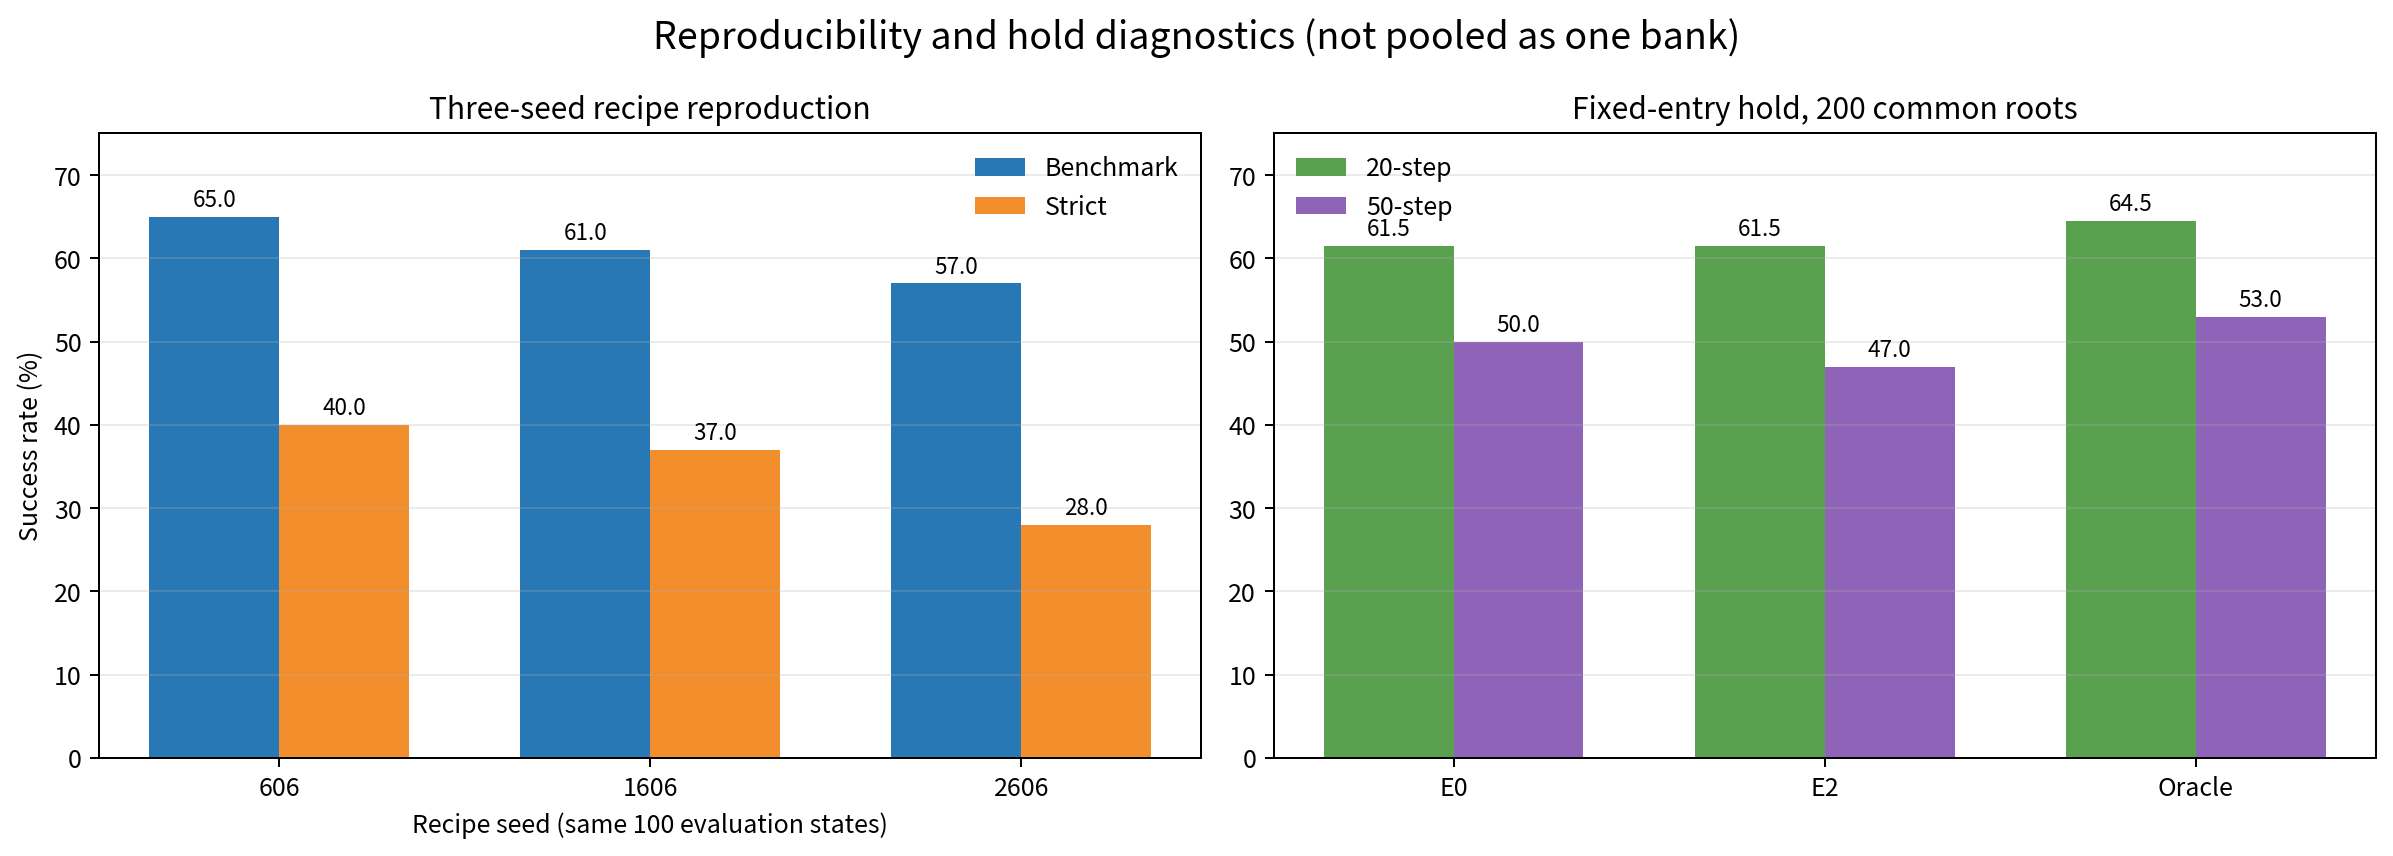
\includegraphics[width=\linewidth]{figures/08_reproduction_and_fixed_hold.png}
\caption{3-seed 复现和 fixed-entry hold}
\end{figure}

\textbf{图 8｜复现性与 hold 诊断。} 左：3 个独立训练 recipe seed 各自在同一组 100 evaluation states 上评测，柱之间反映训练随机性，不能 pooled 成 300 个独立初始状态。右：200 个共同 E0 first-entry roots 的 20/50-step survival，是 paired root 诊断；结果文件未报告 discordance CI。

\hypertarget{ux4e00ux6b21ux6027-200-episode-frozen-test}{%
\subsection{一次性 200-episode frozen test}\label{ux4e00ux6b21ux6027-200-episode-frozen-test}}

frozen test 使用 seeds \texttt{50,000–50,199}。历史 E0 逐 episode 文件与 E2 文件包含完全相同的 200 个 episode ID，可按 ID 连接，因此是 paired test，而不只是两个汇总比例：

\begin{longtable}[]{@{}lrr@{}}
\toprule\noalign{}
Policy & Benchmark & Strict \\
\midrule\noalign{}
\endhead
\bottomrule\noalign{}
\endlastfoot
E0 & 109/200（54.5\%） & 52/200（26.0\%） \\
E2 & 150/200（75.0\%） & 67/200（33.5\%） \\
Difference & \textbf{+20.5pp} & \textbf{+7.5pp} \\
\end{longtable}

Benchmark 有 53 wins、12 losses、135 ties，paired improvement CI \texttt{{[}+13,+28{]}pp}，McNemar \texttt{p=2.79×10\^{}-7}，支持 frozen-test improvement。Strict 有 38 wins、23 losses、139 ties，CI \texttt{{[}0,+15{]}pp}，\texttt{p=0.0722}。由于置信区间下界触及 0，Strict 只能称为方向性提升，不能单独宣称统计显著。

\begin{figure}
\centering
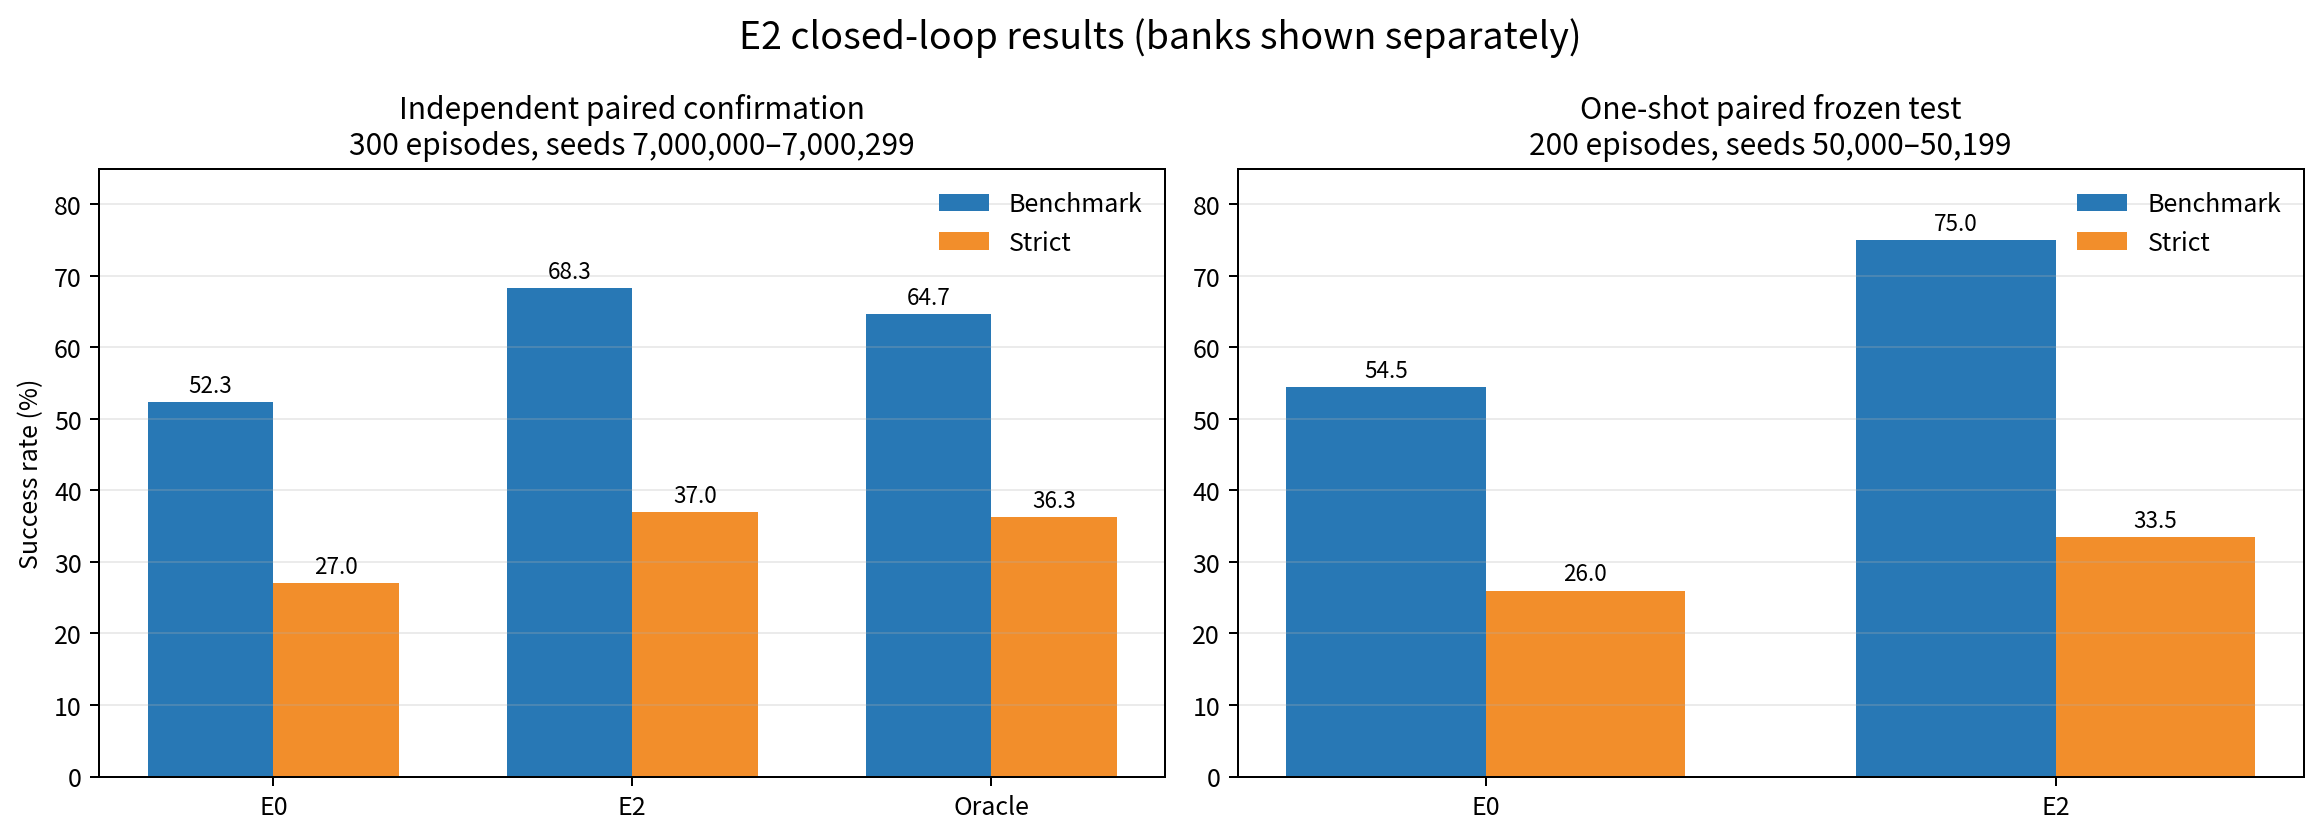
\includegraphics[width=\linewidth]{figures/07_confirmation_and_frozen_test.png}
\caption{独立 confirmation 与 frozen test}
\end{figure}

\textbf{图 9｜最终闭环结果。} 左为 300 个共同 episode seeds 的独立 paired confirmation，右为 200 个共同 episode seeds 的一次性 paired frozen test；两块使用不同 bank，故并排分组而不连线。E2 是在 test 前预选的单一 seed-606 checkpoint，不是 3-seed ensemble，frozen test 没有参与重选或再训练。

frozen test 的角色是最终一次性外部检查，不是又一个开发集。E2 的 75.0\% Benchmark 是本项目最强的最终测试点估计，但不能写成普遍保证；33.5\% Strict 的不确定性仍大，且与 50-step fixed-entry 方向性差距一致地提醒我们：获得目标的能力改善得比长期保持更充分。

\textbf{本章结论。} 独立 300-episode confirmation 为 E2 相对 E0 的 Benchmark 与 Strict 提供了显著 paired 证据，三个训练 seed 复现了收益方向。一次性 frozen test 进一步确认 Benchmark 提升 20.5pp；Strict 提升 7.5pp，但 CI 下界为 0，只能视作方向性结果。E2 是单一预选 checkpoint，不能解释成 ensemble，也不能据有限 bank 宣称普遍超过 Oracle。
